\section{K-Nearest Neighbour (KNN)}

Classification (in a general way) is a supervised learning task in which we try to assign to each sample $x_i$ a \textbf{class label} $y_i$ \arrow the key idea is to separate the feature space in classes.
\vspace{0.2cm}
The goal is to learn a model $f(x)\rightarrow \hat{\prob}(Y=y|X=X)$ and then shift from probabilites to predicting labels \arrow classification is both a prediction problem and a decision problem.

The simplest example of classification model is the \textbf{linear classfier}, which draws a line in the middle of the feature space, dividing the whole data space in two classes.
\begin{figure}[h]
    \centering
    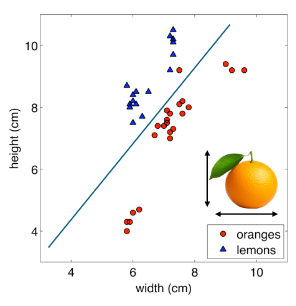
\includegraphics[width=0.2\linewidth]{img//classification//knn/class_lin_example.png}
\end{figure}
The \textit{logistic regression} IS a linar classfier, in fact creates a raw linear division of the log-odds space. The problem is that often the boundaries between classes are non-linear, then requiring to shift toward more complex models \textcolor{gray}{(this idea of dividing the feature space in decisionr regions is common to all classification algorithms)}.

\subsection{K-Nearest Neighbor (KNN)}
The idea behind this is that \textit{similar observations should have similar labels}. 
To classify a new observation we take the $k$-closest training datapoints and predict the new point with the most frequent label. The Euclidean distance is a common choice.
$$
x^* = \arg\min_{x_j\in \text{train set}} d(x_0,x_i)
$$
\vspace{0.2cm}
This type of algorithm is an \textbf{instance-based learning}: the training data is stored and it's actualy used for the prediction. It's also a \textbf{lazy learner}: all the computation is made at prediction time.

\textcolor{green}{\textbf{Pro:}}
\begin{itemize}
    \item extremelly simple
    \item no assumption on the parameters
    \item very flexible, complex shapes may arise
\end{itemize}
\textcolor{red}{\textbf{Cons:}}
\begin{itemize}
    \item extremelly sensitive to noise (one single misprediction might cause huge problems), risk of overfitting
    \item computational expensive at predict time
    \item sensitive to irrelevant features
\end{itemize}

The $k$ at the end is just an hyperparameter and finding the right $k$ is a \textbf{model-selection problem}.
\begin{figure}[h]
    \centering
    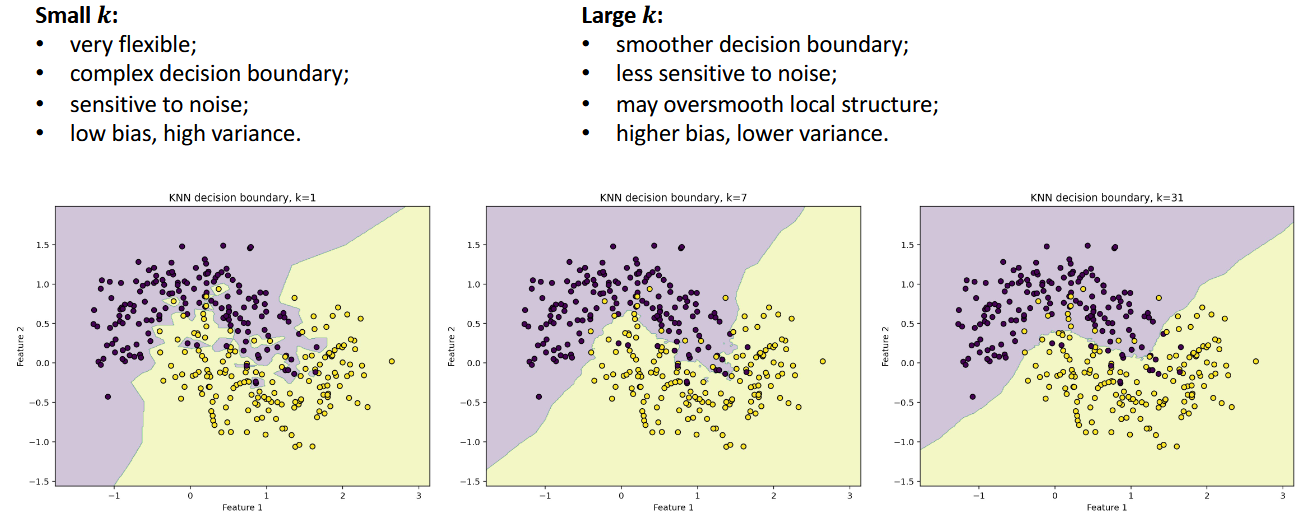
\includegraphics[width=0.5\linewidth]{img//classification//knn/k-neighbour-choice.png}
\end{figure}
